\documentclass[nonacm,sigplan]{acmart}
\settopmatter{printacmref=false}
\usepackage{enumitem}
\usepackage{tabularx}
\usepackage{xcolor}
\usepackage{hyperref}
\usepackage{float}
\usepackage{subcaption}
\usepackage{multicol}
\usepackage{tabularx}
\usepackage{booktabs}
\usepackage{multirow}
\usepackage{array}
\usepackage{siunitx}
\usepackage{listings}
\hypersetup{
  colorlinks=true,
  linkcolor=blue,
  citecolor=red,
  filecolor=magenta,
  urlcolor=cyan
}
\lstset{basicstyle=\ttfamily\footnotesize, breaklines=true}
\definecolor{codebg}{gray}{0.97}
\definecolor{codekw}{rgb}{0.10,0.35,0.70}
\definecolor{codestr}{rgb}{0.60,0.00,0.00}
\definecolor{codecom}{rgb}{0.30,0.50,0.30}

\lstdefinestyle{pystyle}{
  language     = Python,
  basicstyle   = \ttfamily\footnotesize,
  keywordstyle = \color{codekw}\bfseries,
  stringstyle  = \color{codestr},
  commentstyle = \color{codecom}\itshape,
  showstringspaces = false,
  breaklines   = true,
  frame        = single,
  framerule    = 0pt,
  rulecolor    = \color{black!15},
}

\begin{document}
\title[]{MultiModalMan: An Interactive Hangman Game}

\author{Andrea Tarricone}
\email{tarricone.1888181@studenti.uniroma1.it}
\affiliation{%
  \institution{University "La Sapienza"}
  \city{Rome}
  \state{Lazio}
  \country{Italy}
}

\author{Lucian Dorin Crainic}
\email{crainic.1938430@studenti.uniroma1.it}
\affiliation{
  \institution{University "La Sapienza"}
  \city{Rome}
  \state{Lazio}
  \country{Italy}
}

\begin{abstract}
\textbf{MultiModalMan} is a reimagining of the classic \textit{hangman game} that lets players guess letters and control the interface by speaking or using hand gestures as well as by typing. The system is built in \textit{Python} around three modules: a state manager that synchronises all inputs, an \textbf{AI agent} for \textit{natural language processing}, and a \textit{Computer Vision pipeline} for \textit{real time gesture recognition}. Users can switch freely between modalities during play, making the game accessible and engaging for a wide audience. The application is implemented using the \textit{Flet} framework, which provides a responsive web interface that runs in any modern browser. This paper describes the architecture, design patterns, and implementation details of the system, highlighting its innovative use of multimodal interaction to enhance user experience.
\end{abstract}


\begin{teaserfigure}
  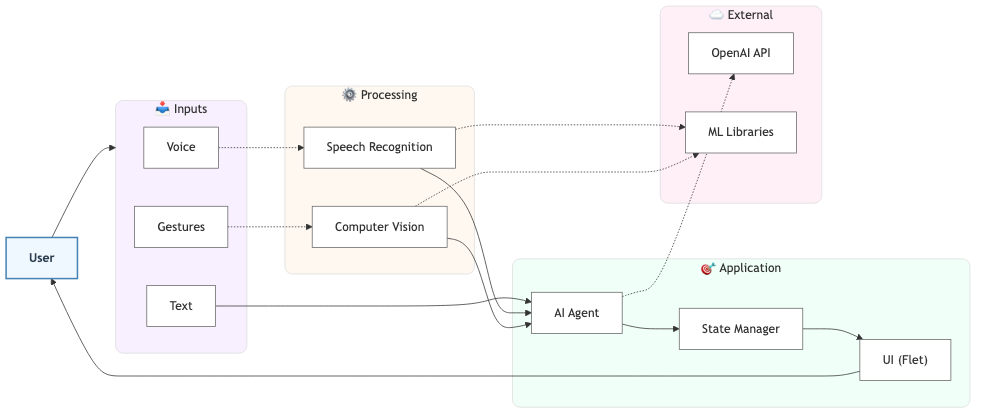
\includegraphics[width=\textwidth]{./images/architecture_diagram.png}
  \caption{High level overview of the MultiModalMan game system showing the flow from user inputs through processing layers to the core application.}
\end{teaserfigure}

\maketitle
\pagestyle{plain}

\section{Introduction}
Digital games have become a mainstream medium for both entertainment and learning, yet they remain unevenly playable. Industry reports estimate that \emph{20–30 \%} of the global player base lives with at least one disability, and almost half of those players already engage with games despite a range of access barriers \cite{ablegamers2024}. Ensuring that games are accessible is therefore both an ethical imperative and a clear educational and commercial opportunity.

Research in multimodal human–computer interaction (HCI) shows that combining complementary input channels—speech, gesture, gaze, or haptics—lowers access barriers and improves task performance. A recent survey notes consistent reductions in error rate, task time, and cognitive load when users can blend modalities rather than rely on a single channel \cite{baig2020}. Game-specific studies echo these findings: gesture-based controllers enable players with motor impairments to execute directional actions that would be impossible on a traditional keyboard \cite{taheri2021}, and experiments that fuse voice commands with hand gestures yield the highest efficiency and perceived naturalness among the tested conditions \cite{cao2023}. Meanwhile, advances in AI speech processing continue to broaden accessibility by adapting to diverse accents and speech differences \cite{morris2019}.

\textbf{MultiModalMan} responds directly to this research agenda. The project re-imagines the classic Hangman game as a language-learning tool that can be played interchangeably through:

\begin{itemize}
  \item spoken commands processed by an AI speech pipeline;
  \item hand-gesture input captured via a webcam and MediaPipe;
  \item conventional keyboard typing.
\end{itemize}

An embedded AI agent maintains the dialogue flow and adapts hints in real time, while a finite-state machine keeps all three modalities synchronised so players can switch fluidly between them without losing context. The project pursues three goals:

\begin{enumerate}
  \item demonstrate how a lightweight multimodal pipeline can be integrated into a small educational game;
  \item provide meaningful accessibility options for users with motor or speech restrictions;
  \item offer a concrete test-bed for the design claims found in multimodal HCI literature.
\end{enumerate}

The remainder of this report details every phase of the project—from refined requirements to architecture, multimodal input handling, interface design, testing, and future work—so that our design decisions remain transparent and reusable.

\section{Aim and Scope}

\noindent
\textit{MultiModalMan} pursues a twofold mission: to illustrate how multimodal interfaces lower accessibility barriers and to turn that insight into an engaging, language-learning game.  Traditional mouse-and-keyboard designs routinely sideline entire user groups.  Blind players cannot perceive graphical feedback; Deaf players can read on-screen text but gain little from audio narration; users with motor impairments may struggle with precise key presses.  By blending speech, gesture and text input, our project offers redundant—and therefore more inclusive—paths through the game.

\subsection{Accessibility Objectives}

\begin{description}[leftmargin=1.2em,style=nextline]
  \item[\textbf{Multiple channels}] Voice, hand gestures and on-screen buttons are interchangeable so that no single sense or motor skill becomes a blocker.
  \item[\textbf{Low reading load}] Visual icons and spoken prompts replace verbose text wherever possible.
  \item[\textbf{Complementarity}] When one modality fails (e.g.\ speech in a noisy room) another can take over without interrupting play.
\end{description}

\subsection{Educational \& Inclusive Goals}

\begin{description}[leftmargin=1.2em,style=nextline]
  \item[\textbf{Broad reach}] Children, language learners and users with motor or speech constraints can all follow the same storyline.
  \item[\textbf{Multisensory learning}] Players reinforce spelling via simultaneous visual, auditory and kinaesthetic cues.
\end{description}

\subsection{Technical Targets}

\begin{description}[leftmargin=1.2em,style=nextline]
  \item[\textbf{Accurate input}] Real-time recognition of spoken letters and hand-drawn glyphs.
  \item[\textbf{Context-aware logic}] An AI agent that interprets free-form utterances and drives adaptive hints.
  \item[\textbf{Unified control}] A central state manager that keeps the three modalities synchronised and responsive.
\end{description}

\section{Requirements}

\subsection{Overview}
The following tables specify the essential capabilities (\textit{Functional}) and quality targets (\textit{Non-Functional}) that \textit{MultiModalMan} must meet to deliver an inclusive, responsive and maintainable gaming experience.

% --------------------------------------------------
\subsection{Functional Requirements}

\begin{table}[h]
\centering
\caption{Functional requirements}
\begin{tabularx}{\linewidth}{@{}lX@{}}
\toprule
\textbf{ID} & \textbf{Description} \\ \midrule
F1 & The user can start a new game at any time. \\
F2 & The system selects a random word from an internal dictionary. \\
F3 & Letters can be guessed through voice commands, hand gestures or keyboard input. \\
F4 & The interface shows the current word state and the number of wrong attempts. \\
F5 & The system announces the outcome (win or loss) when the game ends. \\
F6 & A new round can be launched without restarting the application. \\ \bottomrule
\end{tabularx}
\end{table}

% --------------------------------------------------
\subsection{Non-Functional Requirements}

\begin{table}[h]
\centering
\caption{Non-functional requirements}
\begin{tabularx}{\linewidth}{@{}lX@{}}
\toprule
\textbf{ID} & \textbf{Description} \\ \midrule
NF1 & The user interface must be clear and readable for all age groups. \\
NF2 & The game runs on Windows, macOS and Linux with a standard webcam and microphone. \\
NF3 & Average recognition latency for voice or gesture input is \(\leq\) 2 s. \\
NF4 & Gesture recognition covers the full 26-letter English alphabet\footnote{Or 21 letters for Italian; adjust to the target language set.}. \\
NF5 & The code base is modular and documented to support future extensions. \\
NF6 & The game logic remains consistent when inputs are invalid or ambiguous. \\ \bottomrule
\end{tabularx}
\end{table}

\section{Use Case Model}
A use case captures how an external actor perceives the system.  In \textbf{MultiModalMan} that actor is the \emph{Player}, who may speak, gesture, or type.

\noindent
\textbf{Primary scenarios}\,: UC1 Start Game, UC2 Select Input Mode, UC3 Guess Letter,  
UC4 Display Word State, UC5 Handle End of Game, UC6 Start New Round.

\begin{table}[h]
\centering
\caption{Figure \ref{fig:uc-diagram} displays the UC1 diagram, which illustrates the primary interactions between the Player and the system.}
\begin{tabularx}{\linewidth}{@{}l l X X@{}}
\toprule
\textbf{ID} & \textbf{Actor} & \textbf{Goal} & \textbf{Outcome} \\
\midrule
UC1 & Player  & Launch the application.                    & Home screen shown\\
UC2 & Player  & Choose voice, gesture, or keyboard.        & Selected channel \\
UC3 & Player\textsuperscript{*} & Guess a letter.          & Word state updated \\
UC4 & System  & Present current word and errors.           & Updated status\\
UC5 & System  & Detect win or loss.                        & Outcome announced\\
\bottomrule
\end{tabularx}
\footnotesize\textsuperscript{*}\,Variants:\ Voice\,+STT,\ Gesture\,+CNN,\ or direct keyboard input.
\end{table}

\begin{figure}[h]
  \centering
  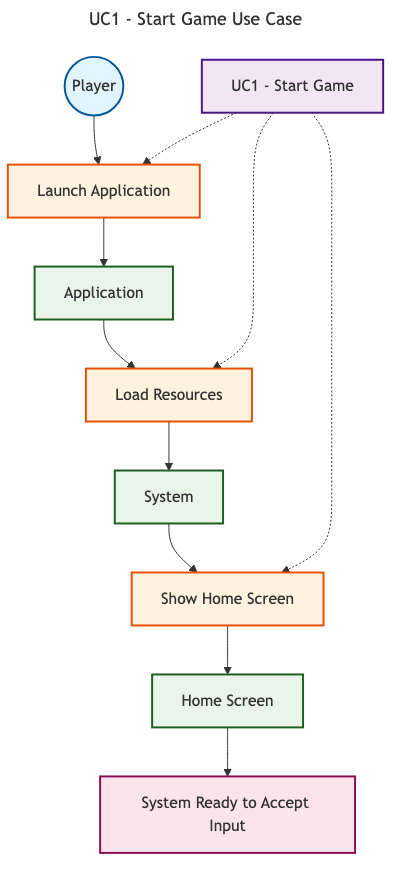
\includegraphics[width=0.3\textwidth]{./images/uc1_start_game.png}
  \caption{Use case diagram for the \textbf{MultiModalMan} game.}
  \label{fig:uc-diagram}
\end{figure}


\section{System Architecture}
The architecture is designed to be cross-platform and independent of the development environment, allowing it to run on Windows, Linux, and macOS systems, provided that a standard webcam and microphone are available.

\subsection{Package Structure}

The application \textit{Hangman 2.0} is designed with a modular architecture, where each package serves a specific and well-defined role within the system. This approach promotes separation of concerns, simplifies code maintenance, and allows for independent development and testing of different functionalities.

At the core of the architecture lies the \texttt{game\_logic} package, which encapsulates the game's main logic: managing the target word, evaluating guesses, tracking errors, and determining win or loss conditions. The \texttt{user\_interface} package is responsible for rendering and updating the graphical user interface, while dynamically reflecting the game state.

The system supports multimodal interaction through two dedicated packages. The \texttt{input\_voice} package handles voice-based input acquisition and processing, leveraging speech recognition technologies. The \texttt{input\_gesture} package manages hand-drawn input captured via webcam and processed through computer vision techniques and a CNN-based classifier.

Lastly, the \texttt{utils} package offers shared support utilities such as logging mechanisms, configuration file handlers, and global constants. This clear packaging strategy enhances modularity and facilitates future scalability.

\subsection{Main Packages Details}

\subsubsection{\texttt{game\_logic}}
This package forms the heart of the application. It includes the \texttt{GameManager} class, which is responsible for the complete management of the hangman game state. It randomly selects a word from a predefined list, keeps track of correct and incorrect guesses, and determines when the game ends.

The class exposes a simple interface to the rest of the system, providing methods such as \texttt{guess\_letter(letter)}, \texttt{is\_game\_over()}, and \texttt{get\_display\_word()} for game interaction. All game-related decision making is centralized in this package.

\subsubsection{\texttt{user\_interface}}
The \texttt{user\_interface} package is tasked with constructing and updating the graphical layout of the application. Depending on the system version, the interface can be implemented using libraries such as \texttt{flet}, \texttt{tkinter}, or \texttt{pygame}. The core class, \texttt{UIManager}, handles the rendering of the current word state, the display of incorrect letters, and the remaining attempts.

It also provides immediate visual feedback to the user's input through animations, color changes, and on-screen messages. Furthermore, it integrates the inputs from various modalities (voice, gesture, keyboard) to ensure a cohesive user experience.

\subsubsection{\texttt{input\_voice}}
This package manages voice-based interaction. Utilizing the \texttt{speech\_recognition} library, it supports multiple backends such as Google Speech API, Whisper, or offline engines. The \texttt{SpeechRecognizer} class handles the acquisition of audio input, the filtering of noise, the transcription of letters, and the resolution of ambiguities.

The module exposes methods such as \texttt{listen\_for\_letter()} and \texttt{get\_last\_result()} to other components, allowing seamless integration into the game loop. Error handling, silence timeouts, and recognition confidence thresholds are incorporated to ensure robustness.

\subsubsection{\texttt{input\_gesture}}
The \texttt{input\_gesture} package enables gesture-based input using computer vision. Through \texttt{OpenCV} and a trained Convolutional Neural Network (CNN), the system recognizes letters drawn in the air by the user's hand.

The \texttt{GestureRecognizer} class is responsible for capturing video frames, applying image preprocessing (such as filtering, detection of the bounding box, and resizing), and performing inference using CNN. It returns the most probable letter detected. The main method, \texttt{capture\_and\_predict()}, encapsulates this entire workflow.

This component is modular and extendable, capable of being re-trained with new datasets or adapted to improved neural architectures for higher accuracy.

\section{Multimodal Interaction}

Multimodal interaction is the cornerstone of \textbf{MultiModalMan}. Instead of locking players into a keyboard and mouse loop, the game accepts spoken commands, hand drawn letters captured by a webcam, and classic text input. A Python state manager keeps these channels in sync, while an OpenAI-powered agent interprets free-form utterances and adapts feedback to the current game phase.

\subsection*{Voice Interaction}
\begin{figure}
    \centering
    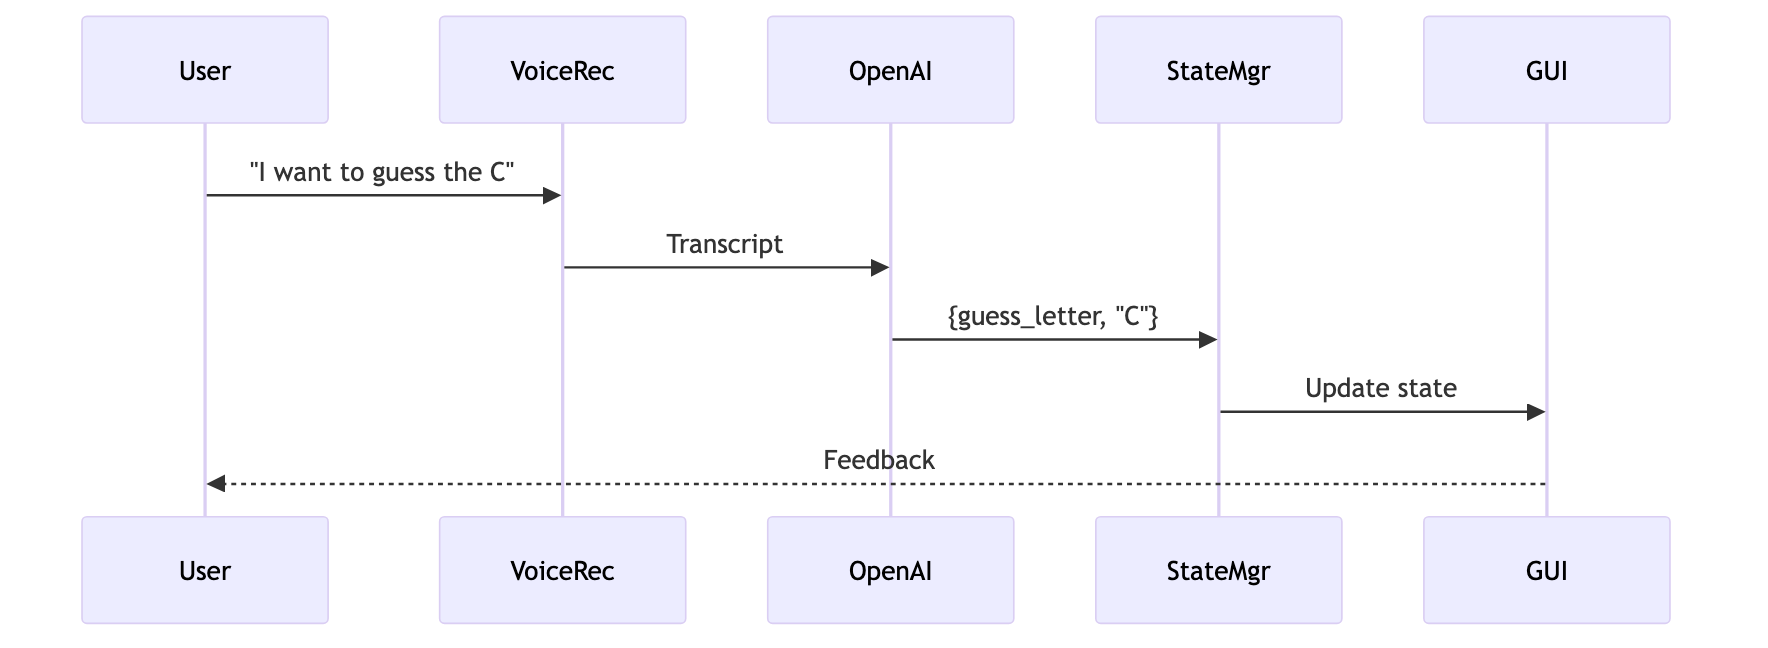
\includegraphics[width=0.55\textwidth]{./images/voice_interaction_flow.png}
    \caption{Activity diagram for the voice interaction component, showing how user speech is processed, transcribed, and routed through the state manager to update the game state.}
\end{figure}
When the user speaks “start game”, “guess C”, or “exit” for instance the audio stream is transcribed in real time (primary engine: \texttt{speech\_recognition}; fallback: Whisper or the Google Speech API). The recognised text is passed to the state manager, which checks whether the utterance is valid for the current state (setup, guessing, or end of game) and routes it accordingly. Natural phrases such as “how many errors do I have?” are interpreted by the OpenAI agent, which converts them into concrete game actions or informational responses.

\subsection*{Gesture Interaction}
\begin{figure}
    \centering
    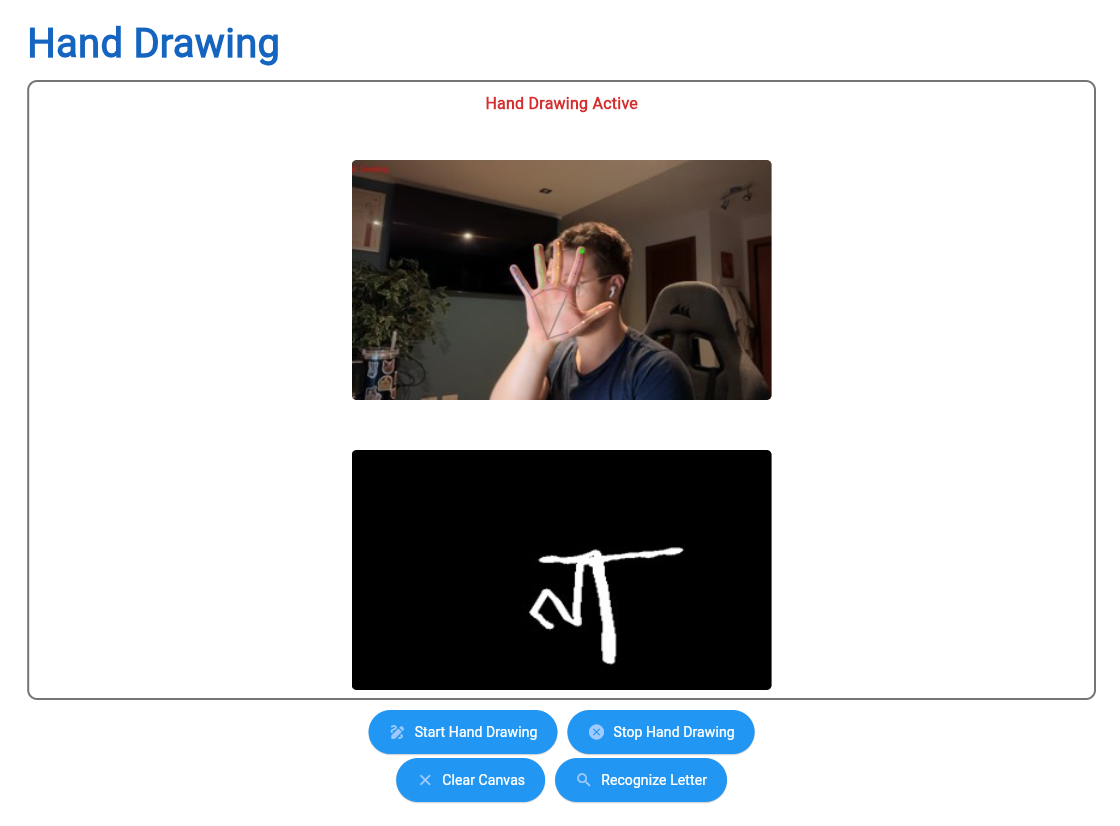
\includegraphics[width=0.55\textwidth]{./images/hand-draw.png}
    \caption{Gesture Interaction in the MultiModalMan game, showing how hand-drawn letters are captured and processed in real time.}
\end{figure}
A webcam continuously detects the user’s hand. OpenCV isolates the region of interest, normalises it, and forwards the image to a lightweight CNN trained on finger spelled letters. The predicted character is then forwarded to the state manager, which decides whether to accept, reject, or request clarification always providing on screen feedback so users understand what was recognised.

\subsection*{State Manager}
\begin{figure}
    \centering
    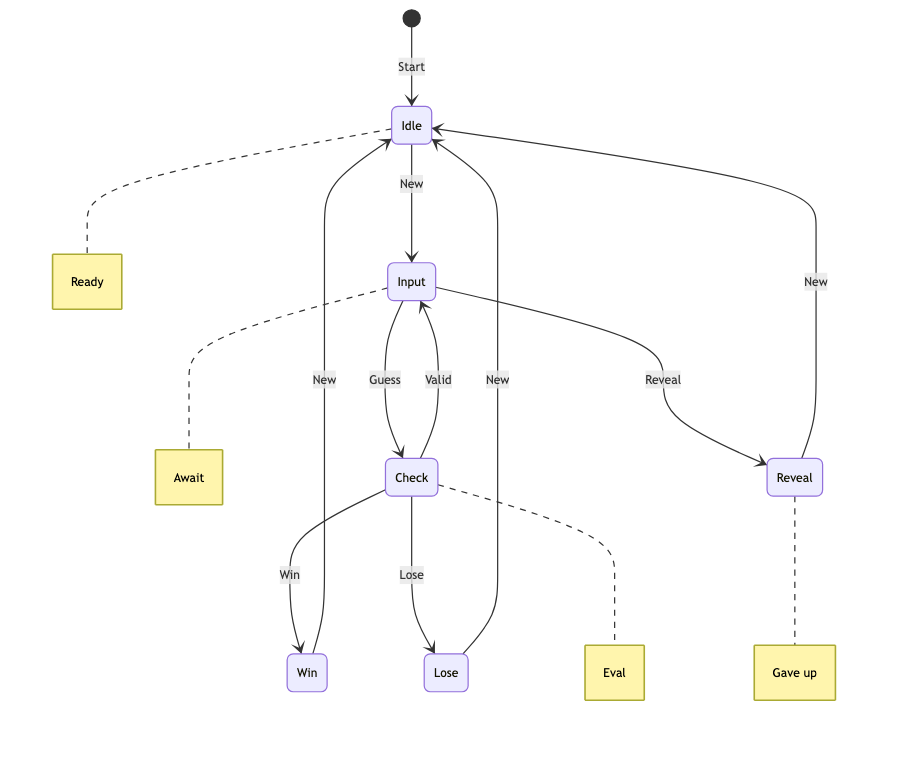
\includegraphics[width=0.5\textwidth]{./images/game_state_manager_state_machine.png}
    \caption{State machine diagram for the \texttt{GameStateManager} class, showing the transitions between different game states based on user inputs and actions.}
    \label{fig:state_machine}
\end{figure}
The \texttt{GameStateManager} class acts as the game’s traffic controller. It tracks a finite set of states (initialisation, waiting for input, verifying, end of game) and exposes two public methods \texttt{handle\_voice\_input()} and \texttt{handle\_gesture()}. Because every modality funnels through this single point, conflicts are resolved centrally: if a gesture and a voice command arrive at the same instant, the manager applies simple time stamping to decide which one to honour first. It also filters commands that make sense only in a given phase (e.g., “new game” is accepted only after a round has finished).

\subsection*{OpenAI Agent}

The agent turns raw language into game intents. It maintains short term context current word, remaining attempts, last hint delivered so that a query like “remind me what I’ve tried” produces a targeted answer.  
Outputs are JSON objects containing an \texttt{action} field (e.g.\ \texttt{"guess\_letter"}) and an optional \texttt{value}.  
This structure lets the state manager treat the agent as just another input device, keeping the architecture loosely coupled.

For security, the OpenAI key is injected via the \texttt{OPENAI\_API\_KEY} environment variable (e.g.\ \texttt{export OPENAI\_API\_KEY=\,$\langle$key$\rangle$} on Unix).

\begin{lstlisting}[style=pystyle,
                   caption={Essential agent scaffold},
                   label={lst:agent}]
agent = Agent(
    name="hangman_game_agent",
    instructions="High-level rules and prompts (truncated for brevity)",
    tools=[
        ("welcome_agent", "Greets and explains rules"),
        ("wordsetter_agent", "Chooses the word"),
        ("letter_guesser_agent", "Processes a letter guess"),
        ("game_restarter_agent", "Starts a new round"),
        ("sync_agent", "Checks active game state"),
    ],
)
\end{lstlisting}

\begin{figure*}[t]
  \center
  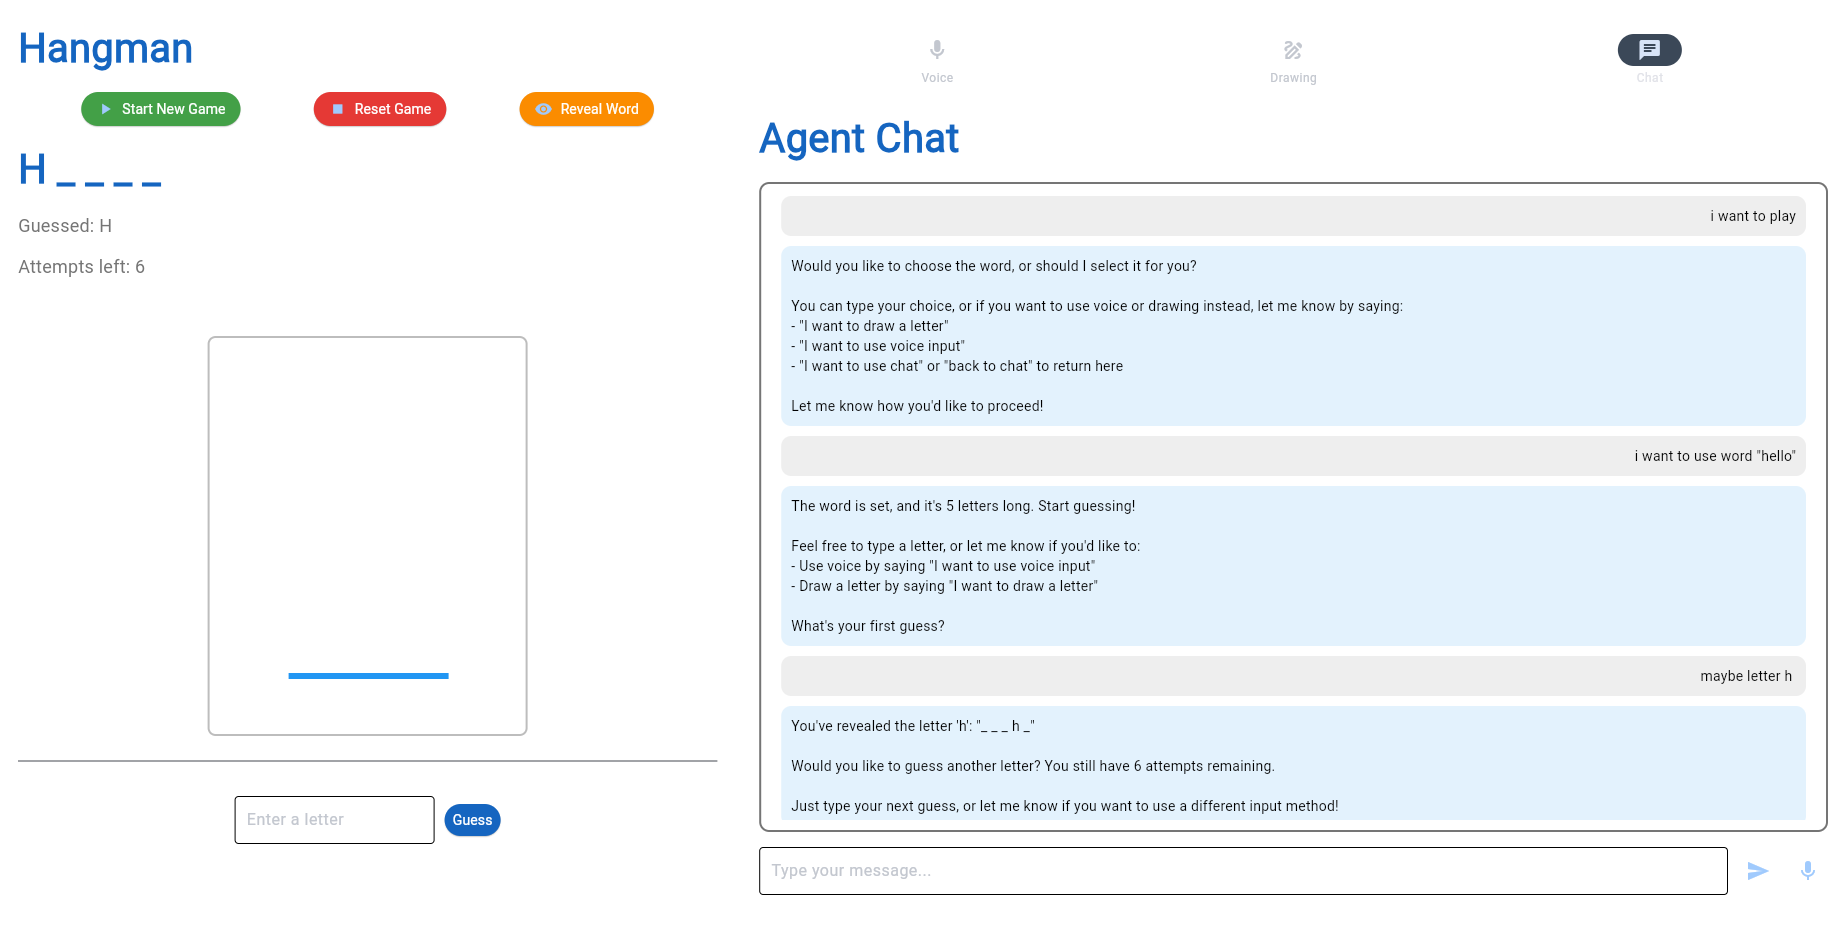
\includegraphics[width=1\textwidth]{images/ui-view.png}
  \caption{Screenshot of the MultiModalMan game interface showing the main game display, hangman visual, and the multimodal input tabs.}
\end{figure*}

\section{GUI Implementation}

\subsection*{Application Architecture}

The GUI is built using the Flet framework, creating a responsive web based interface that runs in the browser. The application follows a two panel layout design where the main game display occupies the left panel and the multimodal input controls are positioned on the right panel.

To launch the application, use the following command from the project root:

\begin{lstlisting}[caption={Starting the Frontend Application}]
flet run frontend/main.py --web
\end{lstlisting}

This opens the game in the default web browser as a responsive web application.

\subsection*{Main Components}

The interface is organized into modular components, each handling specific aspects of the game:

\begin{center}
\begin{tabularx}{\linewidth}{@{}lX@{}}
\toprule
\textbf{Component} & \textbf{Responsibility} \\ \midrule
\texttt{GamePanel}        & Main game interface with word display, hangman visual, and control buttons. \\
\texttt{GameDisplay}      & Shows current word state, guessed letters, remaining attempts, and game status. \\
\texttt{HangmanVisual}    & Animated hangman drawing that progresses with wrong guesses (7 states). \\
\texttt{MediaControls}    & Tabbed interface for voice input, hand drawing, and AI agent chat. \\
\texttt{ManualInput}      & Text input field for manual letter guessing with validation. \\
\texttt{AppLayout}        & Responsive layout manager handling window resizing and notifications. \\ \bottomrule
\end{tabularx}
\end{center}

\subsection*{Game Panel Layout}

The left panel contains the core game interface:

\begin{itemize}
\item \textbf{Control Buttons}: Three action buttons for starting new games, resetting, and revealing words
\item \textbf{Word Display}: Shows the target word with revealed letters or underscores for hidden letters
\item \textbf{Game Information}: Displays guessed letters, remaining attempts, and current game status
\item \textbf{Hangman Visual}: Animated SVG style drawing showing game progress (0-6 wrong guesses)
\item \textbf{Manual Input}: Text field for direct letter input with real time validation
\end{itemize}

\subsection*{Multimodal Input Interface}

The right panel provides three input modalities through a tabbed navigation interface:

\begin{description}
\item[\textbf{Agent Chat}] Natural language conversation with an AI agent that manages the game, processes letter guesses, and provides guidance. Includes voice to text capability for hands free interaction.

\item[\textbf{Voice Input}] Direct voice recognition for letter guessing. Users say "Letter X" to guess a specific letter, with visual feedback showing the recognized input and confidence levels.

\item[\textbf{Hand Drawing}] Computer vision based letter recognition using webcam input. Users draw letters in the air, which are captured, processed through a CNN model, and converted to game guesses.
\end{description}

\subsection*{State Management and Observer Pattern}

The application uses a centralized state management system with an observer pattern for real-time UI updates:

\begin{lstlisting}[style=pystyle, caption={Observer Pattern Implementation}]
class GameStateManager:
    def add_observer(self, callback: Callable[[GameState], None]) -> None:
        """Add a callback function to be called when game state changes"""
        if callback not in self._observers:
            self._observers.append(callback)
    
    def _notify_observers(self, state: GameState) -> None:
        """Notify all observers of a state change"""
        for callback in self._observers:
            callback(state)

# Components register as observers
self.state_manager.add_observer(self.on_state_changed)
\end{lstlisting}

This ensures that all UI components automatically update when the game state changes, whether triggered by manual input, voice commands, hand gestures, or AI agent actions.

\subsection*{Component Implementation Details}

\subsubsection*{GameDisplay Component}

The \texttt{GameDisplay} component handles the visual representation of the current game state:

\begin{lstlisting}[style=pystyle, caption={GameDisplay Update Logic}]
def update(self, state):
    # Handle revealed word display
    if state.game_status == "revealed" and state.secret_word:
        self.word.value = " ".join(state.secret_word)
        self.word.color = config.COLOR_PALETTE["error"]
    else:
        self.word.value = state.display_word
        self.word.color = None
    self._update_status(state)
\end{lstlisting}

\subsubsection*{HangmanVisual Component}

The hangman visual progresses through seven distinct states, from an empty gallows to a complete figure:

\begin{lstlisting}[style=pystyle, caption={Hangman Visual State Management}]
def update_state(self, wrong_guesses):
    """Update the hangman visual based on number of wrong guesses"""
    wrong_guesses = max(0, min(wrong_guesses, 6))
    self.current_state = wrong_guesses
    self.content = self.states[wrong_guesses]
    self.update()
\end{lstlisting}

\subsubsection*{MediaControls Navigation}

The multimodal interface uses a navigation bar to switch between input methods:

\begin{lstlisting}[style=pystyle, caption={Multimodal Interface Navigation}]
def _handle_tab_change(self, e):
    """Handle navigation rail tab change"""
    selected_index = e.control.selected_index
    if selected_index == 0:  # Chat
        self.view_container.content = self.chat_view
    elif selected_index == 1:  # Voice
        self.view_container.content = self.voice_view  
    elif selected_index == 2:  # Drawing
        self.view_container.content = self.drawing_view
    self.view_container.update()
\end{lstlisting}

\section{Conclusion and Future Work}

\subsection{Key Achievements}

\textit{MultiModalMan} re-imagines the classic paper hangman as an inclusive digital game: players can now interact by speaking, gesturing, or typing, while an AI agent orchestrates the state machine, understands natural-language commands, and adapts hints in real time—making the experience accessible to a far wider audience than the original pencil-and-paper version ever reached.

\subsection{Future Directions}
\vspace{-0.5em}
\begin{enumerate}[label=\textbf{F\arabic*}.]
  \item Expand the word set and add text-to-speech for fully voice-driven, multilingual play.
  \item Boost gesture accuracy with larger, augmented datasets and improved CNNs.
  \item Introduce cooperative and time-trial multiplayer modes.
  \item Provide an interactive onboarding sequence for first-time users.
  \item Store user profiles and match history to track learning progress.
\end{enumerate}


\bibliographystyle{ACM-Reference-Format}
\bibliography{references}
\end{document}
